\documentclass[journal,12pt,twocolumn]{IEEEtran}

\usepackage{setspace}
\usepackage{gensymb}
\singlespacing
\usepackage[cmex10]{amsmath}

\usepackage{amsthm}

\usepackage{mathrsfs}
\usepackage{txfonts}
\usepackage{stfloats}
\usepackage{bm}
\usepackage{cite}
\usepackage{cases}
\usepackage{subfig}

\usepackage{longtable}
\usepackage{multirow}

\usepackage{enumitem}
\usepackage{mathtools}
\usepackage{steinmetz}
\usepackage{tikz}
\usepackage{circuitikz}
\usepackage{verbatim}
\usepackage{tfrupee}
\usepackage[breaklinks=true]{hyperref}
\usepackage{graphicx}
\usepackage{tkz-euclide}

\usetikzlibrary{calc,math}
\usepackage{listings}
    \usepackage{color}                                            %%
    \usepackage{array}                                            %%
    \usepackage{longtable}                                        %%
    \usepackage{calc}                                             %%
    \usepackage{multirow}                                         %%
    \usepackage{hhline}                                           %%
    \usepackage{ifthen}                                           %%
    \usepackage{lscape}     
\usepackage{multicol}
\usepackage{chngcntr}

\DeclareMathOperator*{\Res}{Res}

\renewcommand\thesection{\arabic{section}}
\renewcommand\thesubsection{\thesection.\arabic{subsection}}
\renewcommand\thesubsubsection{\thesubsection.\arabic{subsubsection}}

\renewcommand\thesectiondis{\arabic{section}}
\renewcommand\thesubsectiondis{\thesectiondis.\arabic{subsection}}
\renewcommand\thesubsubsectiondis{\thesubsectiondis.\arabic{subsubsection}}


\hyphenation{op-tical net-works semi-conduc-tor}
\def\inputGnumericTable{}                                 %%

\lstset{
%language=C,
frame=single, 
breaklines=true,
columns=fullflexible
}
\begin{document}


\newtheorem{theorem}{Theorem}[section]
\newtheorem{problem}{Problem}
\newtheorem{proposition}{Proposition}[section]
\newtheorem{lemma}{Lemma}[section]
\newtheorem{corollary}[theorem]{Corollary}
\newtheorem{example}{Example}[section]
\newtheorem{definition}[problem]{Definition}

\newcommand{\BEQA}{\begin{eqnarray}}
\newcommand{\EEQA}{\end{eqnarray}}
\newcommand{\define}{\stackrel{\triangle}{=}}
\bibliographystyle{IEEEtran}
\raggedbottom
\setlength{\parindent}{0pt}
\providecommand{\mbf}{\mathbf}
\providecommand{\pr}[1]{\ensuremath{\Pr\left(#1\right)}}
\providecommand{\qfunc}[1]{\ensuremath{Q\left(#1\right)}}
\providecommand{\sbrak}[1]{\ensuremath{{}\left[#1\right]}}
\providecommand{\lsbrak}[1]{\ensuremath{{}\left[#1\right.}}
\providecommand{\rsbrak}[1]{\ensuremath{{}\left.#1\right]}}
\providecommand{\brak}[1]{\ensuremath{\left(#1\right)}}
\providecommand{\lbrak}[1]{\ensuremath{\left(#1\right.}}
\providecommand{\rbrak}[1]{\ensuremath{\left.#1\right)}}
\providecommand{\cbrak}[1]{\ensuremath{\left\{#1\right\}}}
\providecommand{\lcbrak}[1]{\ensuremath{\left\{#1\right.}}
\providecommand{\rcbrak}[1]{\ensuremath{\left.#1\right\}}}
\theoremstyle{remark}
\newtheorem{rem}{Remark}
\newcommand{\sgn}{\mathop{\mathrm{sgn}}}
% \providecommand{\abs}[1]{\left\vert#1\right\vert}
% \providecommand{\res}[1]{\Res\displaylimits_{#1}} 
% \providecommand{\norm}[1]{\left\lVert#1\right\rVert}
% %\providecommand{\norm}[1]{\lVert#1\rVert}
% \providecommand{\mtx}[1]{\mathbf{#1}}
% \providecommand{\mean}[1]{E\left[ #1 \right]}
\providecommand{\fourier}{\overset{\mathcal{F}}{ \rightleftharpoons}}
%\providecommand{\hilbert}{\overset{\mathcal{H}}{ \rightleftharpoons}}
\providecommand{\system}{\overset{\mathcal{H}}{ \longleftrightarrow}}
	%\newcommand{\solution}[2]{\textbf{Solution:}{#1}}
\newcommand{\solution}{\noindent \textbf{Solution: }}
\newcommand{\cosec}{\,\text{cosec}\,}
\providecommand{\dec}[2]{\ensuremath{\overset{#1}{\underset{#2}{\gtrless}}}}
\newcommand{\myvec}[1]{\ensuremath{\begin{pmatrix}#1\end{pmatrix}}}
\newcommand{\mydet}[1]{\ensuremath{\begin{vmatrix}#1\end{vmatrix}}}
\numberwithin{equation}{subsection}
\makeatletter
\@addtoreset{figure}{problem}
\makeatother
\let\StandardTheFigure\thefigure
\let\vec\mathbf
\renewcommand{\thefigure}{\theproblem}
\def\putbox#1#2#3{\makebox[0in][l]{\makebox[#1][l]{}\raisebox{\baselineskip}[0in][0in]{\raisebox{#2}[0in][0in]{#3}}}}
     \def\rightbox#1{\makebox[0in][r]{#1}}
     \def\centbox#1{\makebox[0in]{#1}}
     \def\topbox#1{\raisebox{-\baselineskip}[0in][0in]{#1}}
     \def\midbox#1{\raisebox{-0.5\baselineskip}[0in][0in]{#1}}
\vspace{3cm}
\title{Assignment 2}
\author{Kuntal Sudhir Kokate - EE18BTECH11028}
\maketitle
\newpage
\bigskip
\renewcommand{\thefigure}{\theenumi}
\renewcommand{\thetable}{\theenumi}
Download all latex-tikz codes from 
%
\begin{lstlisting}
    https://github.com/Kkuntal990/C-DS/blob/main/Assignment2/assignment2.tex
\end{lstlisting}

Download all codes from 
\begin{lstlisting}
    
\end{lstlisting}
\section{Problem}
Show that the points $\textbf{A} = \begin{pmatrix} 1 \\ 2 \\ 7 \end{pmatrix}$, $\textbf{B} = \begin{pmatrix} 2 \\ 6 \\ 3 \end{pmatrix}$ and $\textbf{C} = \begin{pmatrix} 3 \\ 10 \\ -1 \end{pmatrix}$ are collinear.
\section{Solution}
We will solve for a general case of given \textbf{n} points of \textbf{m} dimensions.
Check whether three points
\[
    A =
    \begin{pmatrix}
        x_{1}  \\
        x_{2}  \\
        \vdots \\
        x_{n}
    \end{pmatrix},
    B =
    \begin{pmatrix}
        y_{1}  \\
        y_{2}  \\
        \vdots \\
        y_{n}
    \end{pmatrix},
    C =
    \begin{pmatrix}
        z_{1}  \\
        z_{2}  \\
        \vdots \\
        z_{n}
    \end{pmatrix}
\]
are collinear or not.

\subsection{Necessary condition}
Let's take three points \textbf{a}, \textbf{b} and \textbf{c}. We will say that these points are collinear if and only if the $max{|\overrightarrow{AB}|, |\overrightarrow{AC}|, |\overrightarrow{BC}|} = 
\text{sum of other two distances}$. That is, let's say $\overrightarrow{AB}$ is the maximum of three, 
$$\implies \overrightarrow{AB} = \overrightarrow{AC} + \overrightarrow{BC}$$
\subsection{Proof:}
Without loss of generality we can take the above example. Let's say that $\implies \overrightarrow{AB} < \overrightarrow{AC} + \overrightarrow{BC}$, then due to triangle inequality we can say that 
the points \textbf{a}, \textbf{b} and \textbf{c} form a triangle.

\subsection{Example}
Taking our above problem.
 $\textbf{A} = \begin{pmatrix} 1 \\ 2 \\ 7 \end{pmatrix}$, $\textbf{B} = \begin{pmatrix} 2 \\ 6 \\ 3 
\end{pmatrix}$ and $\textbf{C} = \begin{pmatrix} 3 \\ 10 \\ -1 \end{pmatrix}$

\begin{equation}
    |\overrightarrow{AB}| = 5.744
\end{equation}

\begin{equation}
    |\overrightarrow{AC}| = 11.489
\end{equation}

\begin{equation}
    |\overrightarrow{BC}| = 5.744
\end{equation}

Therefore, the points are collinear.

\subsection{Proof by plot}
\begin{figure}[ht]
    \centering
    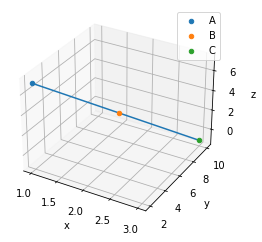
\includegraphics[scale=0.5]{figs/pointsCollinear.png}
    \caption{Plotting the 3 points}
    \label{fig:collinearPoints}
\end{figure}

\end{document}